\chapter{Methodology}
\label{chap:methodology}

This project followed a user centred design methodology to structure the design process to build the chatbot prototype. The process towards building the prototype and its evaluation will be used to answer the research questions:

\begin{enumerate}
    \item Can personality be used as a stable pattern to guide the design process of chatbot interfaces?
    \item How can we design chatbot personalities to guide the design process of a chatbot interface and create a better user experience? 
        \subitem a) Which elements must be considered to inform a chatbot personality?
        \subitem b)What components needs to be in place for a chatbot personality to meet user needs and expectations?
    \item Will the personality be perceived consistently by users?
    \item How can personality be used as a design variable to allow users to perceive them as more than a computer?
        \subitem a) How can designers use personality to improve the conversational design of chatbots? %how can I operationalise conversational design and test this? - can be a simple question in the evaluation
        \subitem b) How will the personality affect the user experience? %metrics consistency, differentiate from similar services, connect relationships with users, motivate - inform hypothesis
\end{enumerate}

The design process will help answer the first research question and sub-questions. As there are no precise design methodology to build user centred chatbots, with a basis in personality, the researcher has combined techniques from user-centred design, branding, and personality theory in order to form a personality framework for chatbot interfaces. This design framework was used to build the chatbot prototype, which was tested and evaluated to answer the research questions regarding the user experience and user perceptions. The evaluation methodology will be laid out after the personality framework has been explained in the next section.

\vspace{5mm} %5mm vertical space

\subsection{Brand, Domain, \& Usage}

To build the chatbot prototype, test the personality framework, and follow a user-centred design approach, the chatbot domain will be based on a real brand. There are no formal collaboration with this brand, therefore it will be anonymised in this thesis. It was necessary to use a real life example to base the prototype on in order to show how the chatbot personality represents the brand's tone of voice, mission and values. This also informed user personas, and suitable users for the chatbot prototype to model the personality on. In addition to this it also informed the role and job the chatbot should have to add value to the user and support the mission of the brand.

The chatbot prototype will be used to further the mission of the brand which is to increase the consumption of fruits and vegetables and reduce food waste. 


\subsection{User group}

The intended user group for the chatbot prototype are between the ages of 25 to 40, aiming at young parents with small or teenage children. As research have found that this age group eats less fruits and vegetables and waste the most food, the chatbot will focus on this age group. This target group usually have hectic days where healthy eating and activity can be difficult to maintain, and they are also in charge of their children’s diet and activity levels as well. As learning good habits starts when we are children, parents have a major impact in regards to teaching children the right habits. Therefore, to support the mission of the brand of increased consumption of fruit and vegetables. People in the age group 25-39 waste more food than other age groups, and in particular families with small children waste more because they have hectic schedules, and little time to plan and prepare meals. This shows that they are in need of a service which can help them cook healthy meals for themselves and their families, learn easy and economical ways to add more nutritious produce to their meals, and learn to waste less food.


\section{Design Process}

The design process was used to investigate techniques and methods to build a user-centred chatbot persona to inform a chatbot prototype. The UCD process was divided into the stages of:  1) inspiration 2) ideation 3) implementation (See Figure 3.0, IDEO.org, 2015). According to \cite{Gould1985} there are three key principles of UCD: an early focus on users and tasks, empirical measurement of product usage, and iterative design. The three stages will therefore all follow the key principles of UCD, where the first stage (inspiration) will focus on user and domain research, ideation will focus on designing the elements of the chatbot prototype, and implementation will focus on the final prototype which will be used to evaluate the design process, the personality framework, and whether personality design benefits the user experience. As a UCD approach is characterised by empirical measurement, iterative design, and focus on users, each deliverable will be empirically tested through user testing techniques in iterations to inform the final prototype.


\vspace{5mm} %5mm vertical space

\subsection{Inspiration phase}

All the stages of the design process followed a strict user-centred design methodology. The inspiration phase focused on gathering insights into the domain at hand. This included conducting a brand analysis of the available content in order to inform the mission statement, values, goals and target audiences. In addition, secondary research was gathered in order to understand trends, causes and action-plans regarding increasing healthier lifestyles and waste less food.

\vspace{2,5mm} %2,5mm vertical space

    \subsubsection{User interviews}
    
    Once secondary knowledge had been collected, a series of interviews was conducted in order to understand the experiences of the users, how do they view their intake of fruit and vegetables, what obstacles do they face, and why they think they are not eating healthy enough. Eight users were recruited, or four couples, in the ages of 29 to 36, four mothers and four fathers. All four couples had two children in kindergarten and/or early elementary school age. Six of the participants works full time, while one mothers was on maternal leave as the interviews were conducted. Two participants, one male and one female, were part-time and/or students at the time of the interviews.
    
    The interview guides prepared were semi-structured and aimed at mapping the daily routines, views, habits, pains and frustrations of the users during an average week. In particular the interviews aimed to see how parents assess their own eating and activity habits, and whether they are aware of food waste occurring and if so why. The interview guide can be found in Appendix XX.
    
    The findings from the interviews were summarised to inform a PACT analysis (appendix XX), to give an understanding of the current state of the services and digital channels of the brand in question and the user group.

\vspace{2,5mm} %2,5mm vertical space

    \subsection{Ideation phase}
    
    In the ideation phase the researcher created user personas, based on findings from the interview and the PACT analysis. To understand the requirements of the system, the user personas describes which goals the users wish to meet using the chatbot, their frustrations and pains and motivations for using the chatbot. Once the personas had been formed, findings from the inspirations phase were used to develop user scenarios --> conceptual scenarios --> concrete scenarios --> use cases. These can be found in Appendix XX.
    
    %show flowchart of how to use scenarios

    
\vspace{5mm} %5mm vertical space

\section{Personality Framework}

The design process, UCD approach, helped form the requirements for the system, define system goals, and use cases. In addition it allowed for valuable insights regarding the users, their needs and frustrations with current solutions. This was necessary to understand the role of the chatbot, and which tasks were necessary for it to do. However, while we know what it needs to do, how can we script the conversation, the different intents, in which the users will have when addressing the chatbot? 

In order to write the chatbot conversation flow, one must be able to understand how the chatbot should behave, and how this behaviour, or personality, best suits the users. To build the personality framework the researcher identified four components that the chatbot personality must be based on:

\begin{enumerate}
    \item The brand mission, goals and values
    \item A deep understanding of the users and their needs
    \item The role/job of the chatbot
    \item An appropriate personality model
\end{enumerate}

These four conditions describes four questions that designers must have the answer to in order to have the necessary components to build the chatbot personality.

\vspace{5mm} %5mm vertical space

    \subsection{The brand mission, goals, and values}
    To design a chatbot that conforms to the brand it represents, the brand image was analysed and defined. The mission statement was identified, the company and core values was defined, and a tone-of-voice analysis was conducted.
    
        \subsubsection{Mission statement and core values}
    
    
        \subsubsection{Tone of Voice analysis}
    
        If the chatbot are to be perceived as an extension or continuation of the brand, it must adhere to the brands tone-of-voice. Tone-of-voice is defined as a brands personality, communicated through its written communication as well as the visual communication. Norman & Nielsen defined a framework to determine tone-of-voice based on 4 dimension: funny vs. serious, formal vs. causal, respectful vs. irreverent, enthusiastic vs. matter-of-fact.
    
        \begin{figure}
            \centering
            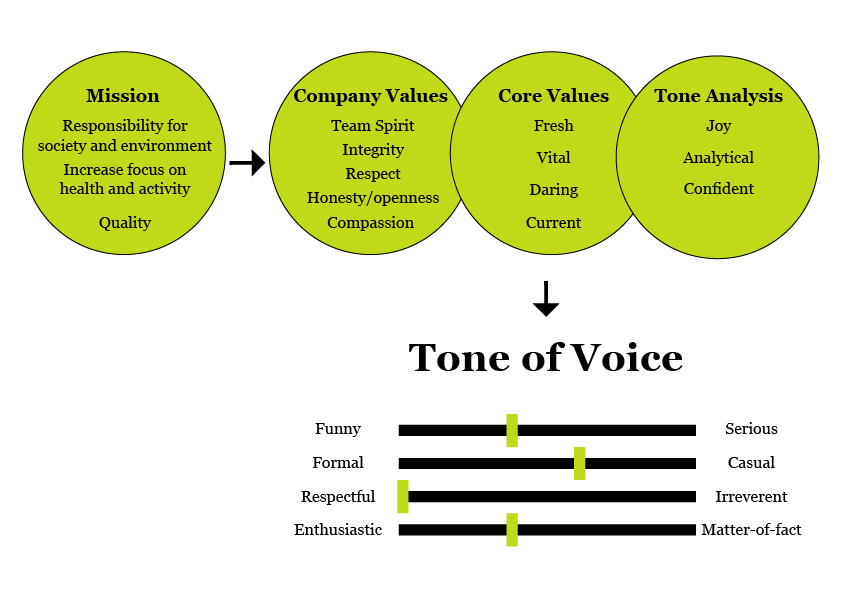
\includegraphics[width=\textwidth]{figures/Tone-of-voice.png}
            \caption{This figure shows how the tone-of-voice was defined by understanding the mission, the values and conducting a tone analysis of the written copy}
            \label{fig:tov}
        \end{figure}
    
        Figure \ref{fig:tov} shows how the tone-of-voice was determined by assessing the mission statement, the company's values inwards and outwards, and through a tone analysis. The tone analysis was conducted using the IBM tone analyser of the written copy found on the brands website. Their tone-of-voice as reflected in their copy is more serious than funny, but not too serious as the tone is also a nice in-between of formal and casual. Their tone is very respectful, which follows their core values of tolerance and respectfulness. Lastly they are leaning towards more enthusiastic than matter-of-fact as they carry a very positive and joyful view of the future and their path to fulfill their goals.

        In addition to the tone-of-voice analysis as proposed by Norman and Nielsen, IBM’s tone analyser tool was also applied to look more into the “mood” they come across as through their web content. The tone analyser searches through content looking for certain words, sentences and phrases that would indicate the mood of the person writing the copy. Their analysis identifies the tones or emotions/mood: anger, fear, joy, sadness, analytical, confident, and tentative. The sentences are then scored and sorted based on how strong they are. If more than one tone is identified in a sentence, then the stronger it is ranked. Four of the tones were identified consistently through the content:
    
        \begin{enumerate}
            \item Analytical
            \item Joy
            \item Confidence
            \item Tentative
        \end{enumerate}

        IBM’s Tone Analyser tool revealed that the tone represented in its online copy consists of: Joy, Analytical, and Confident. In some areas it is also identified as tentative because they are careful in making broad assumptions about its brand: ”We are probably the biggest supplier in Norway”. Rather than tentative a more befitting trait would be humble or realistic. Joy covers any copy where they talks about its achievements, goals and mission - they have a positive outlook and take pride in their achievements towards a healthier population. Analytical is identified where they use numbers and facts to describe their mission and why consumers can trust in their freshness and quality - this is their seriousness in regards to who they are and what they aim to achieve - goal driven and intellectual attitude. Confidence is shown through assertiveness and certainty - they are certain they are on the right path to achieve their goals, and they know that they can help people change. 


    \subsection{Implementation phase}
        \subsection{Conversational Design}
        \subsection{Avatars}
    
    \vspace{5mm} %5mm vertical space
    
    \section{Experiment Setup}
    
    A scenario based test was constructed in order to test the personality of the chatbot and whether the personality affects the user experience. The users will be given a series of tasks testing the most important requirements of the system as revealed through the design process. The test will be used to assess whether the personality is perceived as consistent for all users by implementing the Agree! evaluation method in which compares the given characteristics and personality traits with the agreement of users. The the user experience will be measured by using the AttrakDiff questionnaire to assess the usability and design. 
    
    \vspace{5mm} %5mm vertical space

    \subsection{Hypotheses}
 
    \begin{itemize}
         \item \textit {H11: Chatbot A will have a positive effect on the user experience}
        \item \textit {H10: Personality has no effect on the user experience of chatbots}
            \vspace{5mm} %5mm vertical space

        \item \textit {H21: Users will perceive chatbot A as more consistent than chatbot B}
        \item  \textit {H20: Users will not perceive chatbot A as more or less consistent than chatbot B} 
            \vspace{5mm} %5mm vertical space

        \item \textit {H31: Users will perceive chatbot A more positively than chatbot B}
        \item \textit {H30: Users will not perceive chatbot A more or less positively than chatbot B}
    \end{itemize}
    
    \vspace{5mm} %5mm vertical space
    
    \subsection{Data Collection}
    
    \vspace{5mm} %5mm vertical space

     \subsubsection{Agree!}
     
     In order to evaluate whether the personality is perceived consistently, the participants will be asked to describe the personality in relation to predefined characteristics that are compatible with the chosen personality. The participants will be given a set of characteristics and rate them on whether they perceived or did not perceive that characteristic when interacting with the chatbot. The evaluation will be conducted using the Agree! Tool. This is a software developed by Callejas (2014) that implements the framework for the assessment of synthetic personalities. %site website. 
     
     According to Callejas (2014) Agree! will help evaluate personality in three main dimensions:
    
        \begin{itemize}
            \item Whether the rendered personality is perceived by the users as the designers intended. For example, if the designers plan an extrovert personality, whether users perceive it as extrovert or as something else.
            \item Whether the personality is recognizable, that is, if users perceive it consistently (i.e. if users agree in their perceptions, or different users perceive very different personalities).
            \item Whether the agent's personality matches the users' personality, and how the previous dimensions are affected by the personality of users.
        \end{itemize}
            
    \vspace{5mm} %5mm vertical space
   
     \subsubsection{AttrakDiff}
    
    In order to collect the appropriate data from the test, the AttrakDiff questionnaire was used to assess and compare the two chatbot prototypes. The AttrakDiff assesses personal user rating of a products usability and design. It is an evaluation method that records both the perceived pragmatic quality, the hedonic quality and the attractiveness of an interactive product (cite).
    
        \begin{itemize}
            \item Pragmatic Quality: Usefulness and usability of the system
            \item Hedonic Quality: Motivation, stimulation and challenge for the user
        \end{itemize}
    

   